\def\coursename{量子力学}
\def\courseEnglishname{Quantum Mechanics}
\def\teachername{陈新、郭永}
\def\beginday{2022/3/25}

\documentclass[a4paper, 11pt]{article}

\usepackage[UTF8]{ctex}

\usepackage[T1]{fontenc}								% 字体
\catcode`\。=\active
\newcommand{。}{.} % {\ifmmode\text{.}\else .\fi}
\catcode`\(=\active
\catcode`\)=\active
\newcommand{(}{(}
\newcommand{)}{)}

% \usepackage{zhlineskip}

\usepackage{nicematrix}
% \usepackage{setspace}
% \linespread{1}						% 一倍行距
\setlength{\headheight}{14pt}			% 页眉高度
% \setlength{\lineskip}{0ex}			% 行距
\renewcommand\arraystretch{.82}		% 表格

\usepackage{amssymb, amsmath, amsfonts, amsthm}			% 数学符号,公式,字体,定理环境
\everymath{\displaystyle}			% \textstyle \scriptstyle \scriptscriptstyle
\allowdisplaybreaks[4]      		% 使用行间公式格式
% \makeatletter
% \renewcommand{\maketag@@@}[1]{\hbox{\m@th\normalsize\normalfont#1}}
% \makeatother
\newif\ifcontent\contenttrue		% if 显示目录
\newif\ifparskip\parskipfalse		% if 增加目录后的行距
\newif\ifshowemail\showemailfalse	% if 显示 email
\def\firstandforemost{
	\maketitle
	%\thispagestyle{empty}\clearpage
	\ifcontent
		\renewcommand{\contentsname}{目录}
		\tableofcontents
		\thispagestyle{empty}
		\clearpage
	\fi
	\ifparskip
		\setlength{\parskip}{.8ex}	% 设置额外的段距,目录后
	\fi								% 在 \firstandforemost 前设置 \parskiptrue
	\makenomenclature
	\printnomenclature
	\setcounter{page}{1}
}

\usepackage{mathtools}									% \rcase 环境等

% \usepackage{physics}

\usepackage[]{siunitx}									% 国际制单位
\sisetup{
	inter-unit-product = \ensuremath{{}\cdot{}},
	per-mode = symbol,
	per-mode = reciprocal-positive-first,
	range-units = single,
	separate-uncertainty = true,
	range-phrase = \ifmmode\text{\;-\;}\else\;-\;\fi
}
\DeclareSIUnit\angstrom{\text{Å}}
\DeclareSIUnit\atm{\text{atm}}
% SIunits 额外定义了一个 \square 表示平方,
% 还会把 \cdot 空格加大,真有够无语的 😅

\usepackage{authblk}									% 作者介绍
\ifx \coursefullname\undefined
	\ifx \coursename\undefined
		\def\coursename{笔记}
	\fi
	\def\coursefullname{\coursename}
\fi
\ifx \authorname\undefined
	\def\authorname{Dait}
\fi
\ifx \departmentname\undefined
	\def\departmentname{THU}
\fi
\ifx \emailaddress\undefined
	\def\emailaddress{daiyj20@mails.tsinghua.edu.cn}
\fi
\ifx \beginday\undefined
	\def\beginday{2021}
\fi
\ifx \endday\undefined
	\def\endday{\number\year/\number\month/\number\day}
\fi
\ifx \titleannotation\undefined
	\ifx \teachername\undefined
		\title{\textbf{\coursefullname}}
	\else
		\title{\textbf{\coursefullname}\\\small\textit{主要整理自\teachername 老师讲义}}
	\fi
\else
	\title{\textbf{\coursefullname}\\\small\textit{(\titleannotation)}}
\fi
\newif\ifdefaultauthor\defaultauthortrue
\ifdefaultauthor
	\author{by~\authorname~at~\departmentname}
	\ifshowemail
		\affil{\emailaddress}
	\fi
\fi
\ifx \endday\beginday
	\date{\beginday}
\else
	\date{\beginday~-~\endday}
\fi

\usepackage{hyperref}									% 链接
\ifx \courseEnglishname\undefined
	\def\courseEnglishname{Note}
\fi
\ifx \authorEnglishname\undefined
	\def\authorEnglishname{Dait}
\fi
\hypersetup{
	% dvipdfm								% 表示用 dvipdfm 生成 pdf
	pdftitle={\coursename},
	pdfauthor={\authorname},
	colorlinks=true, breaklinks=true,		% 超链接设置
	linkcolor=black, citecolor=black, urlcolor=blue
}

\usepackage[british]{babel}								% 长单词自动连字符换行
\hyphenation{long-sen-ten-ce}				% 自定义拆分方式

\usepackage{tikz}
\usetikzlibrary{quotes, angles}
\usepackage{pgfplots}
\pgfplotsset{compat=1.17}								% TikZ
\newcommand{\coor}[5][0]{
	\draw[thick,latex-latex](#1,#3)node[left]{$#5$}--(#1,0)node[shift={(-135:7pt)}]{$O$}--(#1+#2,0)node[right]{$#4$}
}			% 坐标轴

\usepackage{enumerate}									% 编号
\usepackage{paralist}
\setlength{\pltopsep}{1ex}
\setlength{\plitemsep}{1ex}
\ifx \eqnrange\undefined
	\numberwithin{equation}{section}
\else
	\numberwithin{equation}{\eqnrange}
\fi

\renewcommand{\thempfootnote}{\Roman{mpfootnote}}
\renewcommand{\thefootnote}{\Roman{footnote}}		% 注释上标 I, II,...
\newcommand{\sectionstar}[1]{
	\section[\hspace{-.8em}*\hspace{.3em}#1]{\hspace{-1em}*\hspace{.5em}#1}
}
\newcommand{\subsectionstar}[1]{					% 带星号的 section 和 subsection
	\subsection{\hspace{-1em}*\hspace{.5em}#1}
}
\newcommand{\subsubsectionstar}[1]{					% 带星号的 section 和 subsection
	\subsubsection{\hspace{-1em}*\hspace{.5em}#1}
}
\newcommand*{\appendiks}{
	\appendix
	\part*{附录}
	\addcontentsline{toc}{part}{附录}
}
\iffalse			% 不清楚
	\newcommand{\varsection}[1]{
		\refstepcounter{section}
		\section*{\thesection\quad #1}
		\addcontentsline{toc}{section}{\makebox[0pt][r]{*}\thesection\quad #1}
	}
\fi

\usepackage{fancyhdr}									% 页眉页脚
\ifx \coursename\undefined
	\def\coursename{笔记}
\fi
\fancyhf{}\pagestyle{fancy}
\fancyhead[L]{\coursename\rightmark}
\fancyhead[R]{by~\authorname}
\fancyfoot[C]{-~\thepage~-} 			%页码

\usepackage{colortbl, booktabs}							% 表

\usepackage{graphicx}
\usepackage{float}
\usepackage{caption}									% 图
\captionsetup{
	margin=20pt, format=hang,
	justification=justified
}
\newcounter{tikzpic}
\def\tikzchap{
	\stepcounter{tikzpic}\\
	\small 图~\thetikzpic\quad
}
\newcounter{linetable}
\newcommand{\tablechap}[1]{
	\stepcounter{linetable}
	{\small 表~\thelinetable\quad #1}\\[1em]
}

\usepackage{tcolorbox}									% 盒子
\tcbuselibrary{theorems, skins, breakable}
\definecolor{MatchaGreen}{HTML}{73C088}		% 抹茶绿B7C6B3
\newtcbtheorem[number within = subsection]{example}{例}{
	enhanced, breakable, sharp corners,
	attach boxed title to top left = {yshifttext = -1mm},
	before skip = 2ex,
	colback = MatchaGreen!5,				% 文本框内的底色
	colframe = MatchaGreen,					% 文本框框沿的颜色
	fonttitle = \bfseries,					% 标题字体用粗体	coltitle 默认 white,
	boxed title style = {
			sharp corners, size = small, colback = MatchaGreen,
		}
}{exm}
\definecolor{MelancholyBlue}{HTML}{9EAABA}	% melancholy: 沮丧
\newcounter{pslt}
\setcounter{pslt}{-1}
\newtcbtheorem[use counter = pslt]{posulate}{假设}{
	enhanced, breakable, sharp corners,
	attach boxed title to top left = {yshifttext = -1mm}, before skip = 2ex,
	colback = MelancholyBlue!5, colframe = MelancholyBlue, fonttitle = \bfseries,
	boxed title style = {
			sharp corners, size = small, colback = MelancholyBlue,
		}
}{psl}
\definecolor{PureBlue}{HTML}{80A3D0}
\newtcbtheorem[number within = subsection]{definition}{定义}{
	enhanced, breakable, sharp corners,
	attach boxed title to top left = {yshifttext = -1mm}, before skip = 2ex,
	colback = PureBlue!5, colframe = PureBlue, fonttitle = \bfseries,
	boxed title style = {
			sharp corners, size = small, colback = PureBlue,
		}
}{dfn}
\definecolor{PeachRed}{HTML}{EA868F}
\newtcbtheorem[number within = subsection]{theorem}{定理}{
	enhanced, breakable, sharp corners,
	attach boxed title to top left = {yshifttext = -1mm}, before skip = 2ex,
	colback = PeachRed!5, colframe = PeachRed, fonttitle = \bfseries,
	boxed title style = {
			sharp corners, size = small, colback = PeachRed,
		}
}{thm}
\definecolor{SchembriumYellow}{HTML}{fbd26a}	% 申博太阳城黄
\newtcbtheorem[number within = section]{method}{方法}{
	enhanced, breakable, sharp corners,
	attach boxed title to top left = {yshifttext = -1mm}, before skip = 2ex,
	colback = SchembriumYellow!5, colframe = SchembriumYellow, fonttitle = \bfseries,
	boxed title style = {
			sharp corners, size = small, colback = SchembriumYellow,
		}
}{mtd}
% 保留颜色
\definecolor{fadedgold}{HTML}{D9CBB0}		% 褪色金
\definecolor{saturatedgold}{HTML}{F0E0C2}	% staurated: 饱和
\definecolor{elegantblue}{HTML}{C4CCD7}		% elegant: 优雅
\definecolor{ivory}{HTML}{F1ECE6}			% 象牙
\definecolor{gloomypruple}{HTML}{CCC1D2}	% 阴沉紫
% \textcolor[HTML]{FFC23A}					% 石板灰

\definecolor{Green}{rgb}{0,.8,0}

\usepackage{imakeidx}								% 索引

\usepackage{nomencl}								% 关键词
%\setlength{\nomitemsep}{0.2cm}							% 设置术语之间的间距
\renewcommand{\nomentryend}{.}							% 设置打印出术语的结尾的字符
\renewcommand{\eqdeclaration}[1]{见公式:(#1)}			% 设置打印见公式的样式
\renewcommand{\pagedeclaration}[1]{见第 (#1) 页}		% 设置打印页的样式
\renewcommand{\nomname}{术语表} 						% 修改术语表标题的名称。

\usepackage{array}
\usepackage{booktabs} % 三线表
\usepackage{multirow}
% 手动排版,尽量杜绝使用

\newcommand{\bs}[1]{\hspace{-#1 pt}}		% 手动减间距	backspace
\newcommand{\bv}[1]{\vspace{-#1 pt}}		% 手动缩行距	backvspace
\def\directlisteqn{\vspace{-1ex}}
\iffalse									% 尽量避免孤行
	\widowpenalty=4000
	\clubpenalty=4000
\fi

% 杂项符号
\def\avg{\overline}
\newcommand*{\rqed}{\tag*{$\square$}}								% 靠右 QED
\newcommand*{\halfqed}{\tag*{$\boxdot$}}
\newcommand*{\thus}{\quad\Rightarrow\quad}							% =>
\newcommand*{\ifnf}{\quad\Leftrightarrow\quad}						% <=>	if and only if
\newcommand*{\turnto}{\quad\to\quad}
\newcommand*{\normalize}{\quad\overset{\mathrm{normalize}}{-\!\!\!-\!\!\!-\!-\!\!\!\longrightarrow}\quad}
\newcommand*{\vthus}{\\$\Downarrow$\\}
\newcommand*{\viff}{\\$\Updownarrow$\\}
\newcommand*{\vs}{~\text{-}~}
\newcommand{\eg}[1][]{\subparagraph*{例#1:}}
\newcommand*{\prf}{\noindent\textbf{证明:}\quad}
\newcommand{\dpfr}[2]{\displaystyle\frac{#1}{#2}}					% 大分数
\newcommand{\frdp}[2]{\frac{\displaystyle #1}{\displaystyle #2}}
\newcommand{\spark}[1]{\;\textcolor{red}{#1}}

% 简化更常用的希腊字母
\newcommand*{\vf}{\varphi}
\newcommand*{\vF}{\varPhi}
\newcommand*{\vp}{\varPsi}
\newcommand*{\ve}{\varepsilon}
\newcommand*{\vC}{\varTheta}
\newcommand*{\ct}{\theta}			% 还是建议用 @ + Tab 快捷键

% 正体符号
\newcommand*{\cns}{\mathrm{const}}
\newcommand*{\plusc}{{\color{lightgray}\,+\,\cns}}
\newcommand*{\e}{\mathop{}\!\mathrm{e}^}	% e
\let\accenti\i
\renewcommand*{\i}{\mathrm{i}}
\newcommand*{\D}{\Delta}
\newcommand*{\p}{\partial}

\usepackage{bm}											% 粗体 \bm
\newcommand{\hbm}[1][r]{\hat{\bm #1}}	% 应该不会有两个字母的
\newcommand{\ibm}[1]{\,\bm #1}

% Using EnglischeSchT script font style
\newfontfamily{\calti}{EnglischeSchT}
\newcommand{\mathcalti}[1]{\mbox{\calti{#1}}}
\newcommand{\mathcaltibf}[1]{\mbox{\bf\calti{#1}}}

\usepackage{mathrsfs}									% 花体 \mathscr
% \usepackage{boondox-cal}								% 小写花体 \mathcal
\newcommand*{\RR}{\mathbb R}
\newcommand*{\CC}{\mathbb C}
\newcommand*{\ZZ}{\mathbb Z}
\newcommand*{\sC}{\mathscr C}			% n 阶连续可导函数
\newcommand*{\sR}{\mathscr R}			% 黎曼可积
% 算符用 \mathcal
\newcommand*{\cL}{\mathcal L}			% 表示一般算子
\newcommand{\cl}[1]{\mathcal L\fkh{#1}}
\newcommand{\cli}[1]{\mathcal L^{-1}\!\fkh{#1}}
\newcommand{\cf}[2][\!\,]{\mathcal F_\mathrm{#1}\fkh{#2}}
\newcommand{\cfi}[2][\!\,]{\mathcal F_\mathrm{#1}^{-1}\!\fkh{#2}}
% \newcommand{\cl}[2][0]{\mathcal L\ikh[#1]{#2}}
% \newcommand{\cli}[2][0]{\mathcal L^{-1}\ikh[#1]{#2}}
% \newcommand{\cf}[2][0]{\mathcal F\ikh[#1]{#2}}
% \newcommand{\cfi}[2][0]{\mathcal F^{-1}\ikh[#1]{#2}}

\usepackage{cancel}										% 删除线

\usepackage{xfrac}

% \usepackage{emoji}	需要 LuaTeX

% 导数等
\let\divides\div
\renewcommand*{\div}{\nabla\cdot}
\newcommand*{\curl}{\nabla\times}
\newcommand*{\lap}{\Delta}
\let\accentd\d
\renewcommand*{\d}{\mathop{}\!\mathrm{d}}
\newcommand*{\nd}{\mathrm{d}}
\newcommand*{\vd}{\mathop{}\!\delta}											% δ
\newcommand{\dd}[2][\;\!\!]{\frac{\nd^{#1}}{\nd #2^{#1}}}						% d/dx			我知道 \,\! 很愚蠢,但是 {} 无法在 Math Preview 上预览
\newcommand{\dn}[2]{\frac{\nd^{#1}}{\nd #2^{#1}}}								% d^n/dx^n		\dn2x≡\dd[2]x
\newcommand{\dv}[3][\;\!\!]{\frac{\nd^{#1}#2}{\nd #3^{#1}}}						% df/dx
\newcommand{\du}[3]{\frac{\nd^{#1}#2}{\nd #3^{#1}}}								% d^nf/dx^n		\du2fx≡\dv[2]fx
\newcommand{\pp}[2][\;\!\!]{\frac{\p^{#1}}{\p #2^{#1}}}							% ∂/∂x
\newcommand{\pn}[2]{\frac{\p^{#1}}{\p #2^{#1}}}									% ∂^n/∂x^n		\pn2x≡\pp[2]x
\newcommand{\pv}[3][\;\!\!]{\frac{\p^{#1}#2}{\p #3^{#1}}}						% ∂f/∂x
\newcommand{\pu}[3]{\frac{\p^{#1}#2}{\p #3^{#1}}}								% ∂^nf/∂x^n		\pu2x≡\pv[2]x
\newcommand{\pw}[3]{\frac{\p^2 #1}{\p #2\p #3}}									% ∂^2f/∂x∂y
\newcommand{\pvv}[6]{															% ∂^(m+n)f/∂x^m∂y^n
	\ifnum#4=1
		\ifnum#6=1
			\frac{\p^{#1}#2}{\p #3\p #5}
		\else
			\frac{\p^{#1}#2}{\p #3\p #5^{#6}}
		\fi
	\else
		\ifnum#6=1
			\frac{\p^{#1}#2}{\p #3^{#4}\p #5}
		\else
			\frac{\p^{#1}#2}{\p #3^{#4}\p #5^{#6}}
		\fi
	\fi}
\newcommand{\dvd}[2]{\left.#1\middle\slash #2\right.}							% 斜除

% 积分
\newcommand*{\intt}{\bs2\int\bs8\int}											% ∫∫
\newcommand*{\inttt}{\int\bs8\int\bs8\int}										% ∫∫∫
\newcommand*{\intdt}{\int\bs3\cdot\bs2\cdot\bs2\cdot\bs4\int}					% ∫...∫
\newcommand*{\zti}{_0^{+\infty}}												% _0^+∞
\newcommand*{\iti}{_{-\infty}^{+\infty}}										% _-∞^+∞
\newcommand{\fmto}[3][\infty]{_{#2=#3}^{#1}}

% 括号
\newcommand{\abs}[1]{\left\lvert#1\right\rvert}									% |x| 绝对值
\newcommand{\norm}[1]{\left\lVert#1\right\rVert}								% ||x|| 模
\newcommand{\edg}[1]{\left.#1\right\rvert}										% f|  竖线
\newcommand{\kh}[1]{\left(#1\right)}											% (x) 括号
\newcommand{\fkh}[1]{\left[#1\right]}											% [x] 方括号
\newcommand{\hkh}[1]{\left\{#1\right\}}											% {x} 花括号
\newcommand{\zkh}[1]{\lfloor\bs{4.7}\lceil #1\rceil\bs{4.7}\rfloor}				% [x] 中括号
\newcommand{\ikh}[2][0]{\ifnum#1=0 \zkh{#2}\else \fkh{#2}\fi}					% [x] 可调大小的中括号
\newcommand{\set}[2]{\left\{#1\,\middle\vert\,#2\right\}}						% {x|x1,x2,...} 集合
\newcommand{\ave}[1]{\left\langle #1\right\rangle}								% <x> 平均值
\newcommand{\bra}[1]{\left\langle #1\right\vert}								% <ψ| 左矢
\newcommand{\ket}[1]{\left\vert #1\right\rangle}								% |ψ> 右矢
\newcommand{\brkt}[2]{\left\langle #1\middle\vert #2\right\rangle}				% <φ|ψ> 内积
\newcommand{\ktbr}[2]{\left\vert#1\right\rangle \bs3\left\langle #2\right\vert}	% |ψ><φ|
\newcommand{\inp}[2]{\left\langle #1,#2\right\rangle}							% <f,g> 内积

% 数学运算符
\let\Real\Re
\let\Imagin\Im
\let\Re\relax
\let\Im\relax
\DeclareMathOperator{\Re}{Re}					% 
\DeclareMathOperator{\Im}{Im}					% 
\DeclareMathOperator{\sech}{sech}				% 
\DeclareMathOperator{\csch}{csch}				% 
\DeclareMathOperator{\arcsec}{arcsec}			% 
\DeclareMathOperator{\arccot}{arccot}			% 
\DeclareMathOperator{\arccsc}{arccsc}			% 
\DeclareMathOperator{\arsinh}{arsinh}			% 
\DeclareMathOperator{\arcosh}{arcosh}			% 
\DeclareMathOperator{\artanh}{artanh}			% 
\DeclareMathOperator{\sgn}{sgn}					% 符号函数
\DeclareMathOperator{\Li}{Li}					% 
\DeclareMathOperator{\Si}{Si}
\DeclareMathOperator{\Ci}{Ci}
\DeclareMathOperator{\sinc}{sinc}
\DeclareMathOperator{\Heaviside}{H}
\DeclareMathOperator{\arr}{A}					% 排列数
\DeclareMathOperator{\com}{C}					% 组合数
\DeclareMathOperator{\Res}{Res}					% 留数
\DeclareMathOperator{\supp}{supp}
\newcommand*{\bigo}{\mathcal O}

% 线性代数
\newif\ifLinearAlgebra\LinearAlgebratrue
\ifLinearAlgebra
\DeclareMathOperator{\rank}{rank}
\DeclareMathOperator{\id}{id}
\newcommand*{\tp}{^{\mathrm T}}				% AT 转置
\newcommand*{\cj}{^\ast}					% A* 共轭
\newcommand*{\dg}{^\dagger}					% A† 共轭转置
\newcommand*{\iv}{^{-1}}					% A-1
\fi

% 物理学家
\newcommand*{\Schr}{Schrödinger}
\newcommand*{\Legd}{Legendre}
\newcommand*{\deB}{de Broglie}
\newcommand*{\Rayl}{Rayleigh}
\newcommand*{\Lande}{Landé}

% 粒子
\newcommand*{\elc}{\mathrm e}
\newcommand*{\pton}{\mathrm p}
\newcommand*{\mol}{\mathrm m}

% 物理常数
\newcommand*{\NA}{N_{\bs1\mathrm A}}						% Avogadro 常数
\newcommand*{\kB}{k_{\mathrm B}}							% Boltzmann 常数
\newcommand*{\muB}{\mu_\mathrm B}							% Bohr 磁矩

% 
\newcommand*{\Ek}{E_{\mathrm k}}							% 动能
\newcommand*{\eff}{_\mathrm{eff}}							% 有效下标
\newcommand*{\tot}{_\mathrm{tot}}
\newcommand*{\lSI}{\tag{SI}}
\newcommand*{\CGS}{\tag{CGS}}								% cm, g, s 制

%\contentfalse

\let\oldr\r
\renewcommand*{\r}{\bm r}						% 坐标向量
\newcommand{\qo}[1]{\bm{\hat #1}\!\mathop{}}	% 量子力学中的向量算符
\newcommand{\cmm}[2]{\zkh{\hat #1,\hat #2}}		% 对易子
\newcommand{\acmm}[2]{\{\hat #1,\hat #2\}}

\newcommand{\Larmor}{\mathrm L}
\newcommand{\Hall}{\mathrm H}

\newcommand{\cyc}{\mathrm c}
\DeclareMathOperator{\Cle}{C}

\begin{document}

%\firstandforemost

\setcounter{section}{6}

\section{自旋}
\subsectionstar{Stern-Gerlach实验}
\begin{center}
	% \usetikzlibrary{arrows.meta} % -Latex
	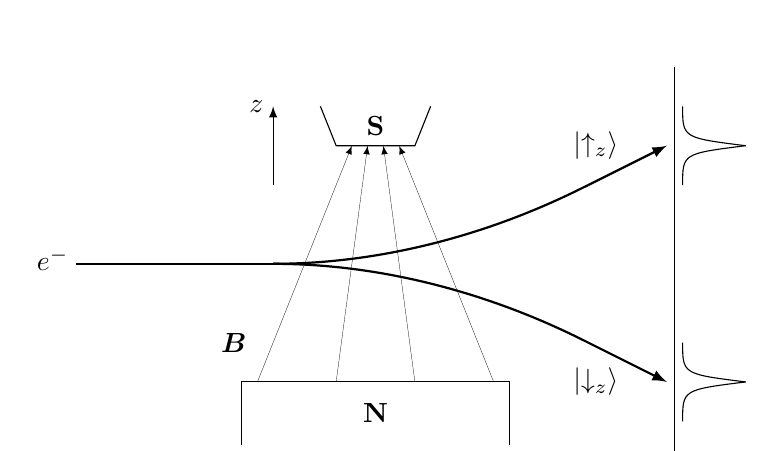
\begin{tikzpicture}
		\draw(0.6,2)--(0.8,1.5)--(1.8,1.5)--(2,2);
		\node at(1.3,1.75){\textbf S};
		\draw[ultra thin,-latex](-.2,-1.5)--(1,1.5);
		\draw[ultra thin,-latex](.8,-1.5)--(1.2,1.5);
		\draw[ultra thin,-latex](1.8,-1.5)--(1.4,1.5);
		\draw[ultra thin,-latex](2.8,-1.5)--(1.6,1.5);
		\draw(-.4,-2.3)--(-.4,-1.5)--(3,-1.5)--(3,-2.3);
		\node at(1.3,-1.9){\textbf N};
		\node at(-.5,-1){$\bm B$};
		\draw[-latex](0,1)--(0,2)node[left]{$z$};
		\node at(-2.8,.06){$e^-$};
		\draw[thick](0,0)--(-2.5,0);
		\draw[thick](0,0)parabola(4,1);
		\draw[thick,-latex](4,1)--(5,1.5);
		\node at(4.1,1.5){$\ket{\uparrow_z}$};
		\draw[thick](0,0)parabola(4,-1);
		\draw[thick,-latex](4,-1)--(5,-1.5);
		\node at(4.1,-1.5){$\ket{\downarrow_z}$};
		\draw(5.1,2.5)--(5.1,-2.5);
		\draw(5.2,1)..controls(5.2,1.4)..(6,1.5);
		\draw(5.2,2)..controls(5.2,1.6)..(6,1.5);
		\draw(5.2,-1)..controls(5.2,-1.4)..(6,-1.5);
		\draw(5.2,-2)..controls(5.2,-1.6)..(6,-1.5);
	\end{tikzpicture}
	\tikzchap Stern–Gerlach实验示意图
\end{center}
% 反常Zeeman效应。

分裂是由于粒子磁矩与磁场相互作用引起的,磁偶极矩在均匀外磁场中的势能
\[V=-\bm\mu\cdot\bm B.\]
在很小线度内非均匀磁场的作用下
\begin{align*}
	\bm F&=-\nabla V=\nabla(\bm\mu\cdot\bm B)\\
	&=(\bm\mu\cdot\nabla)\bm B+\cancel{(\bm B\cdot\nabla)\bm\mu}+\bm\mu\times\cancel{(\curl\bm B)}+\bm B\times\cancel{(\curl\bm\mu)}
\end{align*}
因此磁矩仅在$z$方向上受力
\[\bm F=0+0+\mu_z\pv{B_z}z\bm k.\]

银原子第一激发能$\SI{10.2}\eV$,而热运动能量$\sim\kB T$
\[T=\SI{1e5}\K,\quad \kB T=\SI{8.6}\eV\]
一般实验条件,温度$\ll\SI{e5}\K$,银原子处于基态。只有当磁矩为量子化的(即磁矩在$z$方向的投影量子化)时,条纹才可能是分立的。

银原子在磁场中只有两个取向,有力地证明了原子在磁场中的取向是量子化的。如果角动量空间量子化理论是正确的,要得到偶数个$\mu_z$的值,唯一可能性是角量子数不是整数,而是半整数。说明电子除具有轨道角动量外还应具有自旋角动量。

\subsection{电子自旋}
\paragraph*{电子自旋假设}
\begin{compactenum}
	\item 电子不是质点,有内禀的运动——自旋。%,相应的有自旋角动量和自旋磁矩。
	\item 自旋角动量与轨道角动量类似
		\[\abs{\bm S}=\sqrt{s(s+1)}\hbar.\]
		其中$s$为自旋量子数。
	\item 电子自旋角动量在空间相对外磁场的取向也是空间量子化的,
		\[s_z=\pm\frac{\hbar}2.\]
\end{compactenum}
\paragraph*{自旋的表达}自旋算符$\qo S$和轨道角动量算符$\qo L$具有相同形式关系
\[\qo S=\hat S_x\ibm i+\hat S_y\ibm j+\hat S_z\ibm k.\]
满足角动量算符的共有性质
\begin{gather}
	\qo S\times\,\qo S=\i\hbar\qo S % ,\quad	\cmm{S_x}{S_y}=\i\hbar\hat S_z.
\end{gather}
$\{\hat S^2,\hat S_z\}$的共同本征态$\ket{s,m}$
\begin{align}
	\hat S^2\ket{s,m}&=s(s+1)\hbar^2\ket{s,m},&s&=0,\text{\sfrac12},1,\ldots\\
	\hat S_z\ket{s,m}&=m\hbar\ket{s,m},&m&=-s,-s+1,\ldots,s.
\end{align}
\paragraph*{讨论$s=1/2$}$\qo S$在任意方向上的投影只能取两个数值$\pm\hbar/2$,表象 
\[\ket\updownarrow\equiv\ket\pm:=\ket{\frac12,\pm\frac12}.\]
\paragraph*{Pauli算符}定义 
\[\qo S=\frac\hbar{2}\qo\sigma.\]
有对易关系
\[\qo\sigma\times\,\qo\sigma=2\i\qo\sigma.\]
由$\hat S_x$等的本征值知,$\hat\sigma_x,\hat\sigma_y,\hat\sigma_z$的本征值均为$\pm 1$。

将$\hat\sigma_z\hat\sigma_x-\hat\sigma_x\hat\sigma_z=2\i\hat\sigma_y$分别左、右乘$\hat\sigma_x$,再结合$\hat\sigma_x^2=1$
\begin{align}
	\begin{cases}
		\hat\sigma_x\hat\sigma_z\hat\sigma_x-\hat\sigma_z=2\i\hat\sigma_x\hat\sigma_y\\
		\hat\sigma_z-\hat\sigma_x\hat\sigma_z\hat\sigma_x=2\i\hat\sigma_y\hat\sigma_x
	\end{cases}\thus\hat\sigma_x\hat\sigma_y=-\hat\sigma_y\hat\sigma_x=\i\hat\sigma_z.
\end{align}
或
\begin{align}
	\hat\sigma_\alpha\hat\sigma_\beta=\delta_{\alpha\beta}+\i\sum_\gamma\varepsilon_{\alpha\beta\gamma}\hat\sigma_\gamma.
\end{align}
其中$\varepsilon_{\alpha\beta\gamma}$是Levi-Civita符号。
\paragraph*{自旋算符的矩阵形式-Pauli矩阵}在$\{\hat\sigma^2,\hat\sigma_z\}$表象下
\begin{align}
	\sigma_z=\begin{bmatrix}
		1&0\\0&-1
	\end{bmatrix},
\end{align}
由$\sigma_x\dg=\sigma_x$,$\sigma_x\sigma_z=-\sigma_z\sigma_x$,可设
\[\begin{bmatrix}
	a&b\\b\cj&c
\end{bmatrix}\begin{bmatrix}
	1&0\\0&-1
\end{bmatrix}=-\begin{bmatrix}
	1&0\\0&-1
\end{bmatrix}\begin{bmatrix}
	a&b\\b\cj&c
\end{bmatrix},\]
$a=c=0$,又$\sigma_x^2=1$,可取
\begin{align}
	\sigma_x=\begin{bmatrix}
		0&1\\1&0
	\end{bmatrix},
\end{align}
进而
\begin{align}
	\sigma_y=\i\sigma_x\sigma_z=\begin{bmatrix}
		0&-\i\\\i&0
	\end{bmatrix}
\end{align}
Pauli矩阵都是Hermite的、零迹的、自逆的。
\paragraph*{电子自旋态}电子的旋量波函数(spinor)
\[\psi(\r,t)=\begin{bmatrix}
	\psi_1(\r,t)\\\psi_2(\r,t)
\end{bmatrix}\equiv\psi_1(\r,t)\ket{\uparrow_z}+\psi_2(\r,t)\ket{\downarrow_z}.\]
% 约定$S_z=\pm\hbar/2$的本征态对应$\zkh{1,0}\tp,\zkh{0,1}\tp$。
一般情况,自旋运动和轨道运动有相互作用,此时$\psi_1\neq\psi_2$。当自旋和轨道非耦合时,可以分离出自旋波函数$\chi(s_z)$
\[\psi(\r,t)=\psi_0(\r,t)\chi(s_z).\]

\paragraph*{电子自旋磁矩}实验发现,电子自旋磁矩等于Bohr磁矩
\[\muB=\frac{e\hbar}{2m_\elc},\]
则电子自旋磁矩算符
\[\qo{\mu_s}:=-\frac2\hbar\muB\qo S=-\frac e{m_\elc}\qo S.\]
则
\[\qo{\mu_{sz}}\ket\pm=\mp\muB\ket\pm.\]
轨道磁矩$\qo{\mu_\ell}$和自旋磁矩$\qo{\mu_s}$
\[\qo{\mu_\ell}=g_\ell\frac\muB\hbar\qo L,\quad\qo{\mu_s}=g_s\frac\muB\hbar\qo S,\]
其中旋磁比$g_\ell=-1$,而$g_s=-2$,这是一种相对论效应。
\begin{example}{自旋翻转}{Spin Flip}
	处于恒稳磁场
	\[\bm B=B_0\zkh{\sin\theta\cos\vf,\sin\ct\cos\vf,\cos\ct}\]
	中的电子,$t=0$时处于$\ket{\uparrow_z}$态,求$t>0$自旋翻转的概率。
	
	\textbf{解:}\quad Hamilton量
	\[\hat H=-\qo{\mu_s}\cdot\,\bm B=\muB\qo\sigma\cdot\,\bm B=\muB B_0\begin{bmatrix}
		\cos\ct&\sin\ct\e{-\i\vf}\\\sin\ct\e{\i\vf}&-\cos\ct
	\end{bmatrix},\]
	易得,能量本征值$\pm\muB B_0$,及本征态
	\begin{align*}
		\ket{\uparrow_u}&=\cos\frac\ct{2}\e{-\i\vf/2}\ket{\uparrow_z}+\sin\frac\ct{2}\e{\i\vf/2}\ket{\downarrow_z},\\
		\ket{\downarrow_u}&=-\sin\frac\ct{2}\e{-\i\vf/2}\ket{\uparrow_z}+\cos\frac\ct{2}\e{\i\vf/2}\ket{\downarrow_z}.
	\end{align*}
	将待求波函数按定态展开,
	\begin{align*}
		\psi(0)&=\ket{\uparrow_z}=\cos\frac\ct{2}\e{\i\vf/2}\ket{\uparrow_u}-\sin\frac\theta{2}\e{\i\vf/2}\ket{\downarrow_u};\\
		\psi(t)&=\cos\frac\ct{2}\e{\i\vf/2}\e{-\i\muB B_0t/\hbar}\ket{\uparrow_u}-\sin\frac\theta{2}\e{\i\vf/2}\e{\i\muB B_0t/\hbar}\ket{\downarrow_u}.
	\end{align*}
	因此自旋翻转的概率
	\[\abs{\brkt{\downarrow_z}{\psi}}^2=\sin^2\theta\sin^2\frac{\muB B_0}\hbar t.\]
\end{example}
\subsection{角动量算符}
若矢量算符$\qo J$满足对易关系
\[\qo J\times\,\qo J=\i\hbar\qo J.\]
则称$\qo J$为角动量算符,易证,其平方算符与其分量对易
\[\cmm {J^2}{J_i}=0.\]
取守恒量完全集$\{\hat J^2,\hat J_z\}$,定义升降算符
\begin{align}
	\hat J_\pm:=\hat J_x\pm\i\hat J_y.
\end{align}
注意,升降算符不是Hermite的
\[\hat J_\pm\dg=\hat J_\mp,\]
因此它也不是力学量。

注意到
\begin{align*}
	\hat J_\pm\hat J_\mp&=(\hat J_x\pm\i\hat J_y)(\hat J_x\mp\i\hat J_y)\\
	&=\hat J_x^2\mp\i\cmm{J_x}{J_y}+\hat J_y^2\\
	&=\hat J_x^2+\hat J_y^2\pm\hbar\hat J_z.
\end{align*}
因此 
\begin{align}
	\hat J^2=\hat J_\pm\hat J_\mp+\hat J_z^2\mp\hbar\hat J_z.
\end{align}
\paragraph*{角动量的本征值谱}设$\{\hat J^2,\hat J_z\}$的本征态为$\ket{\lambda,m}$
\begin{align*}
	\hat J^2\ket{\lambda,m}&=\lambda\hbar^2\ket{\lambda,m},\\
	\hat J_z\ket{\lambda,m}&=m\hbar\ket{\lambda,m}.
\end{align*}

由$\cmm{J^2}{J_+}=0$,
\[\bra{\lambda',m'}\cmm{J^2}{J_+}\ket{\lambda,m}=(\lambda'-\lambda)\hbar^2\bra{\lambda',m'}\hat J_+\ket{\lambda,m}=0,\]
因此,只有当$\lambda=\lambda'$时,$\bra{\lambda',m'}\hat J_+\ket{\lambda,m}$才可能不为0:
\begin{align}
	\bra{\lambda',m'}\hat J_+\ket{\lambda,m}=\vd_{\lambda\lambda'}\bra{\lambda,m'}\hat J_+\ket{\lambda,m}.
\end{align}

由$\cmm{J_z}{J_\pm}=\pm\hbar\hat J_\pm$,
\begin{align*}
	\bra{\lambda,m'}\cmm{J_z}{J_\pm}\ket{\lambda,m}&=(m'-m\mp 1)\hbar\bra{\lambda,m'}J_\pm\ket{\lambda,m}\\
	&=\pm\hbar\bra{\lambda,m'}J_\pm\ket{\lambda,m},
\end{align*}
因此$\hat J_\pm$使$m$加、减1:
\begin{align}
	\bra{\lambda',m'}\hat J_\pm\ket{\lambda,m}=\vd_{\lambda\lambda'}\vd_{m\pm 1,m'}\bra{\lambda,m\pm 1}\hat J_\pm\ket{\lambda,m}.
\end{align}

由$\cmm{J_+}{J_-}=2\hbar\hat J_z$,
\[\bra{\lambda,m}\cmm{J_+}{J_-}\ket{\lambda,m}=2m\hbar^2.\]%\vd_{mm'}
插入封闭关系\footnote{下面所有$\lambda$均相同,故略去。}
\begin{align*}
	\sum_{m'}\bra{m}\hat J_+\ktbr{m'}{m'}\hat J_-\ket{m}-\bra{m}\hat J_-\ktbr{m'}{m'}\hat J_+\ket{m}=2m\hbar^2\\
	=\bra{m}\hat J_+\ktbr{m-1}{m-1}\hat J_-\ket{m}-\bra{m}\hat J_-\ktbr{m+1}{m+1}\hat J_+\ket{m}
\end{align*}
由
\[\bra{m-1}\hat J_-\ket{m}=\bra{m}\hat J_+\ket{m-1}\cj\]
上式即
\begin{align}
	\abs{\bra{m}\hat J_+\ket{m-1}}^2-\abs{\bra{m-1}\hat J_+\ket{m}}^2=2m\hbar^2.
\end{align}

令$\bra{m+1}\hat J_+\ket{m}=\xi_m\hbar$,则 
\[\abs{\xi_{m-1}}^2-\abs{\xi_m}^2=2m.\]
解得$\abs{\xi_m}^2=-m(m+1)+\cns.$

因为要求$\abs{\xi_m}^2\geqslant 0$,因此 
\[m(m+1)\leqslant\cns.\]
上式说明$m$存在一个上界$\overline m$和下界$\underline m$,使得
\begin{align*}
	\xi_{\overline m}&=\bra{\overline m+1}\hat J_+\ket{\overline m}=0;\\
	\xi_{\underline m-1}&=\bra{\underline m-1}\hat J_-\ket{\underline m}\cj=0.
\end{align*}
因此$\cns=\overline m(\overline m+1)=(\underline m-1)\underline m$,显然要求$\overline m>\underline m$,故$\overline m=-\underline m=:j$。

由于相邻的$m$相差1,故$j$只能为半整数0, \sfrac12, 1, \sfrac32, $\ldots$,且
\[\abs{\xi_m}^2=j(j+1)-m(m+1)=(j-m)(j+m+1).\]

下面求$\hat J^2$的本征值,对
\[\hat J^2=\frac12(\hat J_+\hat J_-+\hat J_-\hat J_+)+\hat J_z^2\]
取平均值
\[\lambda\hbar^2=\frac{\hbar^2}2\kh{\abs{\xi_{m-1}}^2+\abs{\xi_m}^2}+m^2\hbar^2\]
解得$\lambda=j(j+1)$。

因此$\hat J^2,\hat J_z$是对角矩阵
\begin{align}
	\hat J^2\ket{j,m}&=j(j+1)\hbar^2\ket{j,m},&j&=0,\frac12,1,\frac32,2,\ldots\\
	\hat J_z\ket{j,m}&=m\hbar\ket{j,m},&m&=-j,-j+1,\ldots,j.
\end{align}
比如对于电子的自旋,$j=1/2,m=\pm 1/2$。

而$\hat J_\pm$的矩阵元
\begin{align}
	\hat J_\pm\ket{j,m}=\sqrt{j(j+1)-m(m\pm 1)}\ket{j,m\pm 1}.
\end{align}
\begin{example}{$\hat J_x$的平均值}{Meanvalue of Jx}
	在$\{\hat J^2,\hat J_z\}$的本征态$\ket{j,m}$上
	\begin{align*}
		\bar J_x&=\frac12(\bar J_++\bar J_-)=\frac12\bra{j,m}J_++J_-\ket{j,m}=0.\\
		\avg{J_x^2}&=\frac14\bra{j,m}J_+^2+J_+J_-+J_-J_++J_-^2\ket{j,m}.
	\end{align*}
	$\hat J_y$同理,故
	\begin{align*}
		\bar J_x=\bar J_y&=0,\\
		\avg{J_x^2}=\avg{J_y^2}&=\frac12\kh{\avg{J^2}-\avg{J_z^2}}=\frac{\hbar^2}2\fkh{\ell(\ell+1)-m^2}.
	\end{align*}
\end{example}
\begin{example}{}{}
	基底$\ket{1,-1},\ket{1,0},\ket{1,1}$,为方便略去$j\equiv 1$ %记为$\ket\upuparrows,\ket{\uparrow\downarrow},\ket\downdownarrows$
	\begin{align*}
		J_x=\begin{bmatrix}
			0&\bra{-1}\hat J_x\ket{0}&0\\
			\bra{0}\hat J_x\ket{-1}&0&\bra{0}\hat J_x\ket{1}\\
			0&\bra{1}\hat J_x\ket{0}&0
		\end{bmatrix}
	\end{align*}
	由
	\begin{align*}
		\bra{m\pm 1}\hat J_x\ket{m}&=\frac\hbar{2}\sqrt{j(j+1)-m(m\pm 1)};\\
		\bra{m\pm 1}\hat J_y\ket{m}&=\pm\frac\hbar{2\i}\sqrt{j(j+1)-m(m\pm 1)}.
	\end{align*}
	可得 
	\begin{align*}
		J_x=\frac\hbar{\sqrt2}\begin{bmatrix}
			0&1&0\\1&0&1\\0&1&0
		\end{bmatrix},\quad J_y=\frac{\i\hbar}{\sqrt2}\begin{bmatrix}
			0&1&0\\-1&0&1\\0&-1&0
		\end{bmatrix}.
	\end{align*}
\end{example}
\subsection{角动量合成}
设角动量$\qo{J_1}$和$\qo{J_2}$互相独立,也即它们的分量分别满足角动量的对易关系,而它们互相之间是对易的
\[\cmm{J_{1\alpha}}{J_{2\beta}}=0.\]
则矢量和$\qo J=\qo{J_1}+\qo{J_2}$也是一个角动量算符,称为总角动量,它满足角动量的一般对易关系$\qo J\times\,\qo J=\i\hbar\qo J$。

容易看出$\hat J^2$和$\qo{J_1}$和$\qo{J_2}$并不对易。
\paragraph*{非耦合表象}力学量完全集$\{\hat J_1^2,\hat J_{1z},\hat J_2^2,\hat J_{2z}\}$,基底
\[\ket{j_1,m_1,j_2,m_2}=\ket{j_1,m_1}\otimes\ket{j_2,m_2},\]
也就是说,$\qo{J_1}$只对$\ket{j_1,m_1}$作用,$\qo{J_2}$只对$\ket{j_2,m_2}$作用。

维数$(2j_1+1)(2j_2+1)$,封闭关系
\begin{align*}
	\sum_{m_1=-j_1}^{j_1}\sum_{m_2=-j_2}^{j_2}\ktbr{j_1,m_1,j_2,m_2}{j_1,m_1,j_2,m_2}=I.
\end{align*}
\paragraph*{耦合表象}力学量完全集$\{\hat J_1^2,\hat J_2^2;\hat J^2,\hat J_z\}$,基底
\[\ket{j_1,j_2,j,m}\]
封闭关系
\[\sum_{j=j_{\min}}^{j_{\max}}\sum_{m=-j}^j\ktbr{j_1,j_2,j,m}{j_1,j_2,j,m}=I.\]
\paragraph*{非耦合/耦合表象间基底变换}对于确定的$j_1$和$j_2$,在$(2j_1+1)(2j_2+1)$维空间中
\begin{align*}
	\ket{j_1,j_2,j,m}=\sum_{m_1=-j_1}^{j_1}\sum_{m_2=-j_2}^{j_2}\ket{j_1,m_1,j_2,m_2}\bs3\brkt{j_1,m_1,j_2,m_2}{j_1,j_2,j,m},
\end{align*}
定义矢量耦合系数Clebsch-Gordan系数
\[\Cle_{j_1m_1j_2m_2}^{jm}=\brkt{j_1,m_1,j_2,m_2}{j_1,j_2,j,m}\]
则
\begin{align}
	\ket{j_1,j_2,j,m}=\sum_{m_1=-j_1}^{j_1}\sum_{m_2=-j_2}^{j_2}\Cle_{j_1m_1j_2m_2}^{jm}\ket{j_1,m_1,j_2,m_2}
\end{align}
\paragraph*{总角动量本征值谱}对于确定的$j_1$和$j_2$,总角量子数$j$的取值系列为
\begin{align}
	j=\abs{j_1-j_2},\ldots,j_1+j_2
\end{align}
由$\hat J_z=\hat J_{1z}+\hat J_{2z}$
\begin{align*}
	\hat J_z\ket{j_1,j_2,j,m}=m\hbar\ket{j_1,j_2,j,m}=m\hbar\sum_{m_1,m_2}\Cle_{j_1m_1j_2m_2}^{jm}\ket{j_1,m_1,j_2,m_2};\\
	\begin{aligned}
		(\hat J_{1z}+\hat J_{2z})\ket{j_1,j_2,j,m}&=(\hat J_{1z}+\hat J_{2z})\sum_{m_1,m_2}\Cle_{j_1m_1j_2m_2}^{jm}\ket{j_1,m_1,j_2,m_2}\\
		&=(m_1+m_2)\hbar\sum_{m_1,m_2}\Cle_{j_1m_1j_2m_2}^{jm}\ket{j_1,m_1,j_2,m_2}.
	\end{aligned}
\end{align*}
由$\ket{j_1,m_1,j_2,m_2}$正交归一,$m=m_1+m_2$。% \qed

故$j_{\max}=m_{\max}=m_{1\max}+m_{2\max}=j_1+j_2$,又表象变换不改变维数
\[\sum_{j=j_{\min}}^{j_{\max}}2j+1=(2j_1+1)(2j_2+2)\thus j_{\min}=\abs{j_1-j_2}.\rqed\]
\subsection{碱金属原子能谱的双线结构和Zeeman效应}
碱金属原子($_3$Li, $_{11}$Na等%, $_{19}$K, $_{37}$Rb, $_{55}$Cs
)中的原子实\footnote{原
子核及内层满壳电子,比如Li$^+$。}比较稳定,低激发能级来自价电子的激发。价电子的Hamilton量
\begin{align}
	\hat H_0=-\frac{\hbar^2}{2\mu}\nabla^2+V(r).
\end{align}
屏蔽Coulomb场
\[V(r)=-\frac{e^2}r-\lambda\frac{ae^2}{r^2},\quad 0<\lambda\ll 1.\]

非耦合表象:力学量完全集$\{\hat H_0,\hat L^2,\hat L_z,\hat S^2,\hat S_z\}$,有 % 能量本征值问题的解
\[\hat H_0\ket{n,\ell,m_\ell,m_s}=E_{n\ell}^0\ket{n,\ell,m_\ell,m_s},\]
表达式中略去了电子自旋$s\equiv$\ \sfrac12。其简并度$2(2\ell+1)$.

耦合表象:$\{\hat H_0,\hat L^2,\hat S^2,\hat J^2,\hat J_z\}$,有 
\[\hat H_0\ket{n,\ell,j,m_j}=E_{n\ell}^0\ket{n,\ell,j,m_j}.\]
\paragraph*{自旋-轨道耦合项}
除了Coulomb作用外,价电子的自旋磁矩还受到来自电子轨道运动的内磁场的作用。内磁场很强,一般$\sim10$~T。电子的自旋磁矩与内磁场的相互作用能(Thomas项)
\begin{align}
	\hat H_{LS}=\xi(r)\qo L\cdot\,\qo S%=\frac12\xi(r)\kh{\hat J^2-\hat L^2-\hat S^2}.
\end{align}
%通过繁琐的电磁学计算,或
通过Dirac方程并取非相对论极限可知
\[\xi(r)=\frac1{2\mu^2c^2}\frac1r\dv{V}r.\]
$\hat H_{LS}$对能级的贡献很小,但能引起能级劈裂,形成能谱的双线结构。在原子核的壳结构中,核子之间的强自旋轨道耦合起着极其重要的作用。

为使
\[\hat H=\hat H_0+\hat H_{LS}=\hat H_0+\frac12\xi(r)\kh{\hat J^2-\hat L^2-\hat S^2}\]
最大限度对角化,力学量完全集应该包括尽量多的与$\hat H$对易的算符,由于非耦合表象中的$\hat L_z,\hat S_z$与$\hat J^2$不对易,故选取非耦合表象基底来计算$\hat H$的矩阵元。

用对角矩阵元近似代表能级
\begin{align*}
	E_{n\ell j}&\doteq\bra{n,\ell,j,m_j}\hat H\ket{n,\ell,j,m_j}\\
	&=E_{n\ell}^0+\frac{\hbar^2}2\fkh{j(j+1)-\ell(\ell+1)-\frac34}\bra{n,\ell,j,m_j}\xi(r)\ket{n,\ell,j,m_j}
\end{align*}
而
\begin{align*}
	&\bra{n,\ell,j,m_j}\xi(r)\ket{n,\ell,j,m_j}\\
	&=\sum_{s_z}\sum_{s_z'}\int\brkt{n,\ell,j,m_j}{\r,s}\bs3\bra{\r,s}\xi(r)\ket{\r',s'}\brkt{\r',s'}{n,\ell,j,m_j}\d^3r\d^3r'
\end{align*}
其中 
\begin{align*}
	\brkt{\r,s}{n,\ell,j,m_j}&=R_{n\ell}(r)\sum_{m_\ell,m_s}\Cle_{\ell m_\ell sm_s}^{jm_j}Y_\ell^{m_\ell}(\theta,\varphi)\chi_{m_s}(s_z);\\
	\bra{\r,s}\xi(r)\ket{\r',s'}&=\xi(r)\vd(r-r')\vd(\theta-\theta')\vd(\varphi-\varphi')\vd_{s,s'}.
\end{align*}
故
\begin{align*}
	\bra{n,\ell,j,m_j}\xi(r)\ket{n,\ell,j,m_j}&=\int\zti R_{n\ell}(r)\xi(r)R_{n\ell}(r)r^2\d r%\sum_{m_\ell m_s}\abs{\Cle_{\ell m_\ell sm_s}^{jm_j}}^2\\
	=\ave\xi_{n\ell}.
\end{align*}
计及$\hat H_{LS}$后碱金属原子的能级
\[E_{n\ell j}\doteq E_{n\ell}^0+\frac{\hbar^2}2\fkh{j(j+1)-\ell(\ell+1)-\frac34}\ave\xi_{n\ell}\]

$\ell\neq 0$时,$j=\ell\pm 1/2$,能级分裂为两条
\[E_{n\ell j}\doteq E_{n\ell}^0+\begin{cases}
	\frac{\hbar^2}2\ell\ave\xi_{n\ell},& j=\ell+\frac12\\
	-\frac{\hbar^2}2(\ell+1)\ave\xi_{n\ell},& j=\ell-\frac12
\end{cases}\]
自旋角动量和轨道角动量平行的态的能量比反平行态的能量高。

$\ell=0$时,$j=1/2$不分裂。
\paragraph*{正常Zeeman效应}1896年,Zeeman做实验发现原子在外磁场中发光谱线一分为三的现象,称为Zeeman效应。他的老师Lorentz利用电子论\footnote{用到了中学学到的Lorentz力。}对此给出了理论解释,1902年二人共同获得Nobel物理学奖。

在外磁场下价电子的Hamilton量(忽略$\hat H_{LS}$)
\[\hat H=\hat H_0+\frac{\muB B_0}\hbar(\hat L_z+2\hat S_z),\]
非耦合表象中$\hat H$是对角化的,
\[E_{n\ell m_\ell m_s}=E_{n\ell}^0+\muB B_0(m_\ell+2m_s).\]
外磁场破坏了原子的球对称性,使能级关于磁量子数的简并完全消除。%下图表示Na黄线的正常塞曼效应,跃迁的选择定则为

跃迁的选择定则为
\[\D\ell=\pm 1,\quad \D m_\ell=0,\pm 1,\quad \D m_s=0.\]
注意:跃迁只在$s=1/2$或$s=-1/2$两组能级内部进行,而不允许$s=\pm 1/2$间跃迁。
因此每条光谱线都分裂为三条,间隔相同。
\paragraph*{反常Zeeman效应}后来又发现了比三条谱线更复杂的分裂现象,称为反常Zeeman效应。这是因为在外磁场较弱时不能忽略$\hat H_{LS}$
\[\hat H=\hat H_0+\hat H_{LS}+\frac{\muB B_0}\hbar(\hat J_z+\hat S_z).\]
由于$\hat J^2$与$\hat S_z$不对易,第三项矩阵元关于$j$不对角,但因磁场$B_0$较小,可取对角矩阵元近似
\[E_{n\ell jm_j}\doteq E_{n\ell j}+\omega_\Larmor\kh{m_j\hbar+\bra{n\ell jm_j}\hat S\ket{n\ell jm_j}}\]
换基底得
\[\bra{n\ell jm_j}\hat S\ket{n\ell jm_j}=\hbar\sum_{m_\ell m_s}\abs{\Cle_{\ell m_\ell sm_s}^{jm_j}}^2m_s=\hbar\sum_{m_s}\abs{\Cle_{\ell,m_\ell-m_s,sm_s}^{jm_j}}^2m_s.\]
由
\subsection{自旋单态、三重态及纠缠态}
\paragraph*{单体近似下两个电子的自旋函数}
两电子体系,自旋自由度为2。可选择$\{\hat S_{1z},\hat S_{2z}\}$为自旋力学量的完全集,也可以选$\{\hat S^2,\hat S_z\}$为自旋力学量完全集。

单体近似下,忽略两个电子间的s-s耦合。两电子的自旋函数$\chi(s_{1z},s_{2z})$是每个电子自旋函数$\chi_\alpha(s_z)$之积
\[\chi(s_{1z},s_{2z})=\chi_{m_s}(s_{1z})\chi_{m'_s}(s_{2z}),\quad s_1=s_2=\frac12,\quad m_s=m'_s=\pm\frac12.\]

无耦合表象$\{\hat S_{1z},\hat S_{2z}\}$的基底$\ket{\uparrow\uparrow},\ket{\uparrow\downarrow},\ket{\downarrow\uparrow},\ket{\downarrow\downarrow}$,有对称自旋函数
\[\ket{\uparrow\uparrow},\ket{\downarrow\downarrow},\ket{\updownarrow}:=\frac1{\sqrt2}\kh{\ket{\uparrow\downarrow}+\ket{\downarrow\uparrow}}\]
及反对称函数
\[\ket\Updownarrow :=\frac1{\sqrt2}\kh{\ket{\uparrow\downarrow}-\ket{\downarrow\uparrow}}\]
这四个构成正交归一系。下面证明,他们也是$\{\hat S^2,\hat S_z\}$的本征态。

两电子体系的总角动量平方算符
\begin{align*}
	\hat S^2=(\qo{S_1}+\qo{S_2})^2=\hat S_1^2+\hat S_2^2+2(\hat S_{1x}\hat S_{2x}+\hat S_{1y}\hat S_{2y}+\hat S_{1z}\hat S_{2z})
\end{align*}
又
\begin{gather*}
	S_z\ket\uparrow=\frac\hbar{2}\ket\uparrow,\quad S_z\ket\downarrow=\frac\hbar{2}\ket\downarrow,\\
	S_x\ket\uparrow=\frac\hbar{2}\begin{bmatrix}0&1\\1&0\end{bmatrix}\begin{bmatrix}1\\0\end{bmatrix}=\frac\hbar{2}\ket\downarrow,\quad S_x\ket\downarrow=\frac\hbar{2}\ket\uparrow\\
	S_y\ket\uparrow=\frac\hbar{2}\begin{bmatrix}0&-\i\\\i&0\end{bmatrix}\begin{bmatrix}1\\0\end{bmatrix}=\frac{\i\hbar}{2}\ket\downarrow,\quad \quad S_y\ket\downarrow=-\frac{\i\hbar}{2}\ket\uparrow.
\end{gather*}
故
\begin{align*}
	S\ket{\uparrow\uparrow}&=\frac34\hbar^2\ket{\uparrow\uparrow}+\frac34\hbar^2\ket{\uparrow\uparrow}+2\sum S_{1\alpha}\ket\uparrow S_{2\alpha}\ket\uparrow\\
	&=\kh{\frac34+\frac34+0+0+\frac12}\hbar^2\ket{\uparrow\uparrow}=2\hbar^2\ket{\uparrow\uparrow},\\
	S_z\ket{\uparrow\uparrow}&=S_{1z}\ket{\uparrow\uparrow}+S_{2z}\ket{\uparrow\uparrow}=\hbar\ket{\uparrow\uparrow}.
\end{align*}
因此四个态
\begin{align*}
	\chi_{11}&:&S\ket{\uparrow\uparrow}&=2\hbar^2\ket{\uparrow\uparrow}&S_z\ket{\uparrow\uparrow}&=\hbar\ket{\uparrow\uparrow}\\
	\chi_{1-1}&:&S\ket{\downarrow\downarrow}&=2\hbar^2\ket{\downarrow\downarrow},&S_z\ket{\downarrow\downarrow}&=-\hbar\ket{\downarrow\downarrow};\\
	\chi_{10}&:&S\ket\updownarrow&=2\hbar^2\ket\updownarrow,&S_z\ket\updownarrow&=0;\\
	\chi_{00}&:&S\ket\Updownarrow&=0,&S_z\ket\Updownarrow&=0.
\end{align*}
可作为耦合表象$\{\hat S_1^2,\hat S_2^2,\hat S^2,\hat S_z\}$的基底

自旋三重态:两电子自旋相互平行的态是三重简并的;自旋单态:两电子自旋相互反平行的态是单一的。
\paragraph*{纠缠态}
由两个粒子组成的复合体系的量子态,可表示为每个粒子的量子态的乘积,称为可分离态,如$\chi_{11},\chi_{1-1}$;反之则为纠缠态,如$\chi_{10},\chi_{00}$。
\end{document}